%%%%%%%%%%%%%%%%%%%%%%%%%%
%%%%%%%%%%%%%%%%%%%%%%%%%%
%%%%%% HEADER	 %%%%%%%%%
%%%%%%%%%%%%%%%%%%%%%%%%%%
%%%%%%%%%%%%%%%%%%%%%%%%%%
%%%%%%%%%%%%%%%%%%%%%%%%%%

\documentclass{article}

\usepackage{amsmath}
\usepackage{amsthm}
\usepackage{amssymb}
\usepackage{bbm}
\usepackage{fancyhdr}
% \usepackage{listings}
\usepackage{cite}
\usepackage{graphicx}
\usepackage{enumitem}
\usepackage{courier}
\usepackage[pdftex,colorlinks=true, urlcolor = blue]{hyperref}


\oddsidemargin 0in \evensidemargin 0in
\topmargin -0.5in \headheight 0.25in \headsep 0.25in
\textwidth 6.5in \textheight 9in
\parskip 6pt \parindent 0in \footskip 20pt

% set the header up
\fancyhead{}
\fancyhead[L]{Stanford Computer Science}
\fancyhead[R]{Winter 2020}

%%%%%%%%%%%%%%%%%%%%%%%%%%
\renewcommand\headrulewidth{0.4pt}
\setlength\headheight{15pt}

\usepackage{xparse}
\NewDocumentCommand{\codeword}{v}{%
\texttt{\textcolor{blue}{#1}}%
}

\usepackage{xcolor}
\setlength{\parindent}{0in}

%%%%%%%%%%%%%%%%%%%%%%%%%%
%%%%%%%%%%%%%%%%%%%%%%%%%%
%%%%%% TITLE	 %%%%%%%%%
%%%%%%%%%%%%%%%%%%%%%%%%%%
%%%%%%%%%%%%%%%%%%%%%%%%%%
%%%%%%%%%%%%%%%%%%%%%%%%%%

\title{CS 237B: Principles of Robot Autonomy II \\ Problem Set X}
\author{Name:      \\ SUID:}
\date{}

\begin{document}

\maketitle
\pagestyle{fancy} 

%%%
%% PICTURE
%\begin{figure}
%\begin{center}
%\includegraphics[width=13cm,keepaspectratio]{""}
%\caption{}
%\label{fig:fignum}
%\end{center}
%\end{figure}
%%%

%%%%%%%%%%%%%%%%%%%%%%%%%%
%%%%%%%%%%%%%%%%%%%%%%%%%%
%%%%%% P1		 %%%%%%%%%
%%%%%%%%%%%%%%%%%%%%%%%%%%
%%%%%%%%%%%%%%%%%%%%%%%%%%
%%%%%%%%%%%%%%%%%%%%%%%%%%


\section*{Problem 1}
\begin{enumerate}[label=(\roman*)]
\item
A form closure grasp has a more constrained requirement than a force closure grasp. The concept of form closure implies the object is kinematically constrained, meaning it is impossible to move the object with any external wrench or disturbance. Form closure will typically achieve this by having more contacts, enveloping the object to prevent disturbances. Under form closure, the joint angles of the gripper are locked and a force does not even need to be applied by the contacts. Force closure implies a grasp can be maintained to resist any potential external wrench or disturbance, by providing force and utilizing friction. This means that by satisfying the requirement of form closure, the requirement for force closure is also satisfied.
\item There is requirement for $n + 1$ vectors to positively span a space $\mathbb{R}^n$. For a 2D object, the wrench space is $\mathbb{R}^3$ and hence we need $3 + 1 = 4$ contact points. Similarly, for the 3D object, the wrench space is $\mathbb{R}^6$ (the 3 linear and 3 angular components) meaning we need $7$ contact points.

To elaborate with an example, there will always exist a wrench (or vector in the wrench space) which the $n$ wrenches do not compensate for. For example, consider the 2D case, where 3 wrenches exist:

\begin{align}
\omega_1 &= \begin{bmatrix}
1 \\
0 \\
0 \\
\end{bmatrix}, &
\omega_2 &= \begin{bmatrix}
0 \\
1 \\
0 \\
\end{bmatrix}, &
\omega_3 &= \begin{bmatrix}
0 \\
0 \\
1 \\
\end{bmatrix} 
\end{align}
In this case, assuming the linear combination of the wrenches require scalars $\beta_{k} > 0$, it is clear that a wrench like $\omega_4 = [-1, -1, -1]$ is necessary to ensure the grasp can apply a zero wrench for all external wrenches. This follows with the definition of form closure, as $\omega_4$ is not linearly independent from the other wrenches. It also is equivalent to saying the wrench space has to contain the origin in its interior. This should also be clear  that it is trivial to demonstrate the same for the 3D case.

\item An image is attached showing the wrench hull diagrams. These can be used to estimate the validity of removing one of the point contacts. 

TODO: write valid contacts

TOOD: tau is estimated based on the distances from the center of mass. It is clear that the distance from center of mass to a point is greatest at the far corners of the triangle, while being shortest at the perpendicular to the edges. Using basic geometry we can calculate the minimum and maximum line length and estimate the magnitude of tau at some value in between, based on visual inspection of the diagram. 

%%
% PICTURE
\begin{figure}
\begin{center}
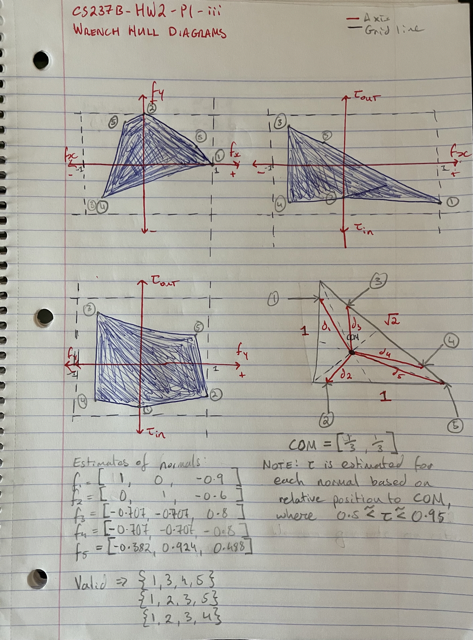
\includegraphics[width=13cm,keepaspectratio]{"images/P1iii.png"}
\caption{Wrench Hull Diagrams for (iii)}
\label{fig:P1iii}
\end{center}
\end{figure}
%%

\item See code.

\item See code.

\item TODO:

\end{enumerate}

%%%%%%%%%%%%%%%%%%%%%%%%%%
%%%%%%%%%%%%%%%%%%%%%%%%%%
%%%%%% P2		 %%%%%%%%%
%%%%%%%%%%%%%%%%%%%%%%%%%%
%%%%%%%%%%%%%%%%%%%%%%%%%%
%%%%%%%%%%%%%%%%%%%%%%%%%%



\section*{Problem 2}
\begin{enumerate}[label=(\roman*)]
\item
\item

\end{enumerate}


%%%%%%%%%%%%%%%%%%%%%%%%%%
%%%%%%%%%%%%%%%%%%%%%%%%%%
%%%%%% P3		 %%%%%%%%%
%%%%%%%%%%%%%%%%%%%%%%%%%%
%%%%%%%%%%%%%%%%%%%%%%%%%%
%%%%%%%%%%%%%%%%%%%%%%%%%%

\section*{Problem 3}
\begin{enumerate}[label=(\roman*)]
\item See code.
\item

\end{enumerate}

\end{document}